\documentclass[aspectratio=169]{beamer}
\usetheme[sectiontoc]{montreal}

\pgfplotsset{
	compat=1.8,
	discrete axis/.style={
		width=0.95\textwidth,
		height=3.5cm,
		enlargelimits=false,
		axis lines=left,
		major tick length=1mm,
		grid=both,
	},
	extra tick style={
		grid style={
			red,
			dashed
		}
	},
	%%%%%%%%%%%%%%%
	% Data labels %
	%%%%%%%%%%%%%%%
	pcirc/.style={
		ylabel=Pcirc (hPa),
		table/x index=0,
		table/y index=2
	},
	debit/.style={
		ylabel=Débit (l/m),
		table/x index=0,
		table/y index=3
	},
	eadi/.style={
		ylabel=Edi (µV), 
		table/x index=0,
		table/y index=5
	},
	poes/.style={
		ylabel=Poes (hPa)
	},
	paw/.style={
		ylabel=Paw (hPa)
	},
	pdi/.style={
		ylabel=Pdi (hPa)
	},
	emgdi/.style={
		ylabel=EMGdi (µV), 
	},
}

\tikzset{
	highlight/.style={
		fill=vertchum, 
		opacity=.42
	},
}

\newenvironment{imgframe}{%
	\setbeamercolor{normal text}{bg=black!92, fg=white}
	\begin{frame}
		\centering
}{%
	\end{frame}
}

\def\imgframe#1{%
	\begingroup
	\setbeamercolor{normal text}{bg=black!92, fg=white}
	\begin{frame}
		\centering
		\includegraphics[height=\pageheight]{#1}
	\end{frame}
	\endgroup
}

\setbeamertemplate{footline}[frame number]

\def\fnote#1{\footnote[1]{#1}}
\def\adapte#1{\fnote{\em Adapté de \cite{#1}.}}
\def\tire#1{\fnote{\em Tiré de \cite{#1}.}}


\subtitle{Enjeux reliés à la filtration du signal EMGdi}
\title{Zones d'ombre du NAVA}
\date{20 juillet 2022}
\institute{\noihu\\[0.1\baselineskip]\papp}
\titlebg{captures/220515_113919.png}
\addbibresource{filtration.bib}

\begin{document}

\maketitle

\begin{frame}{Discussion\footnote{\emph{Avec des restants de vieux
nouveau logo}}}
	\vspace{-2.0cm}
	\begin{minipage}{0.4\textwidth}
		\centering
	\rvnl[fill=bleuclairchum!50]{Avez vous parfois l'impression que\\ le NAVA \emph{ne
fonctionne pas} ?}\\
	\end{minipage}
	\hspace{1.5cm}
	\begin{minipage}{0.4\textwidth}
		\vspace{4cm}
		\rvnl[draw=turquoisechum, fill=turquoisechum!40]{Lâche moi avec
			ton *@!\#\% de NAVA ! \\Y-a dix minutes, j'étais
		encore accroché \\ sur la porte des toilettes...}
	\end{minipage}
\end{frame}

\begin{frame}[label=406]{La catastrophe !}
	\begin{tikzpicture}[
		zonedecompte/.style={
			fill=turquoisechum,
			opacity=0.15
		}
		]
		\begin{groupplot}[
			discrete axis,
			group style={
				group size=1 by 3,
				vertical sep=5mm
			}
			]
			\nextgroupplot[pcirc]
			\addplot table {data/1652614813406-parsed.dat};
			\nextgroupplot[debit]
			\addplot table {data/1652614813406-parsed.dat};
			\nextgroupplot[eadi]
			\addplot table {data/1652614813406-parsed.dat};
			\coordinate (A) at(0,0);
			\coordinate (B) at(axis cs:6,\pgfkeysvalueof{/pgfplots/ymax});
			\coordinate (C) at(axis cs:0,13);
			\coordinate (D) at(axis cs:6,13);
		\end{groupplot}

		\fill<2>[zonedecompte] (A) rectangle (B);
		\draw<2>[
			%bleufoncechum!70!white,
			turquoisechum,
			shorten <=0.5mm,
			shorten >=0.5mm,
			<->,
			%thick,
			font=\scriptsize
			]
			(C) -- (D) node[midway, above] {6 sec.};
	\end{tikzpicture}
\end{frame}



\maketoc

\section{Filtration du signal EMGdi}

\usetikzlibrary{backgrounds}
\begin{frame}{Électromyogramme du diaphragme}
	\framesubtitle{{\color<2>{vertchum}Signal} et {\color<3->{red}Bruit}}

	\begin{tikzpicture}[
		eadihl/.style={
			thick,
			fill=vertchum,
			fill opacity=0.4
		}
		]
		\begin{axis}[
			discrete axis,
			emgdi,
			height=0.5\textheight,
			hide x axis,
			]
			\addplot graphics[points={(0,-150)(100,150)}]{jonkman/jonkman_b_emgdi-250_250};

		\end{axis}

		\foreach \x in {1.3, 4.2, 7.3, 10.35}{%
			\visible<2>{%
				\fill[eadihl] (\x, 1.3cm) ellipse[x radius=5mm, y radius=12mm]; 
		}};
	\fill<4>[
		red,
		opacity=0.4
	] (0,1.25cm) rectangle (11.7,1.45cm);

		\foreach \x in {.22, .763, ..., 12}{%
			\uncover<3>{\node[red, font=\small] at(\x, -.2cm) {$\uparrow$};}
		}
	\end{tikzpicture}\adapte{jonkman_inadequate_2020}
\end{frame}

\begin{frame}{Électromyogramme du diaphragme}
	\centering

	\begin{tikzpicture}[
		fleche/.style={
			vertchum,
			->,
			ultra thick,
			shorten <=2mm,
			shorten >=2mm
		},
		filtre/.style={
			draw,
			pos=0.5,
			vertchum,
			ultra thick,
			fill=white
		},
		]

		\begin{groupplot}[
			discrete axis,
			height=0.45\textheight,
			width=0.45\textwidth,
			hide x axis,
			axis line shift=0,
			group style={
				group size=2 by 1,
				horizontal sep=3cm
			}
			]
			\nextgroupplot[title=EMGdi (µV)]
			\addplot graphics[points={(0,-150)(100,150)}, includegraphics={clip, trim=0 0 4cm 0},]{jonkman/jonkman_b_emgdi-250_250};

			\nextgroupplot[title=Edi (µV)]
			\addplot graphics[points={(0,-0)(100,30)}, includegraphics={clip, trim=0 0 4cm 0},]{jonkman/jonkman_b_eadi-0_50};
		\end{groupplot}
		
		\path (group c1r1.east)--(group c2r1.west) node[filtre] (F) {Filtre};
		\draw [fleche] (group c1r1.east) -- (F) ;
		\draw [fleche] (F) -- (group c2r1.west) ;

	\end{tikzpicture}\\[5mm]
	\adapte{jonkman_inadequate_2020}
\end{frame}

\begin{frame}{Signal brut et filtré}

	\begin{tikzpicture}[]
		\begin{axis}[
			discrete axis,
			legend pos=outer north east,
			legend cell align=left,
			legend style={draw=none, fill=none},
			height=0.65\textheight,
			width=0.9\textwidth,
			hide x axis,
			]
			\addplot graphics[points={(0,-150)(100,150)}]{jonkman/jonkman_b_emgdi-250_250};
			\addplot[red]
			graphics[points={(0,0)(100,30)}]{jonkman/jonkman_b_eadi-0_50-clear};

		\legend{EMGdi (µV), Edi (µV)}
	\end{axis}
		
\end{tikzpicture}
\adapte{jonkman_inadequate_2020}
\end{frame}


\section{Filtration incomplète}

\begin{frame}{Électromyogramme du diaphragme}
	\centering

	\begin{tikzpicture}[
		]

		\begin{groupplot}[
			discrete axis,
			height=0.40\textheight,
			width=\textwidth,
			hide x axis,
			group style={
				vertical sep=5mm,
				group size=1 by 3,
			},
			]
			\nextgroupplot[eadi]
			\addplot graphics[
				points={(0,-0)(100,50)}
				]{jonkman/jonkman_b_eadi-0_50};

			\nextgroupplot[emgdi]
			\addplot graphics[
				xmin=0,
				xmax=100,
				ymin=-250,
				ymax=250,
				]{jonkman/jonkman_b_emgdi-250_250};

				\only<3>{
			\nextgroupplot[pdi]
			\addplot graphics[
				xmin=0,
				xmax=100,
				ymin=-5,
				ymax=25,
				]{jonkman/jonkman_b_pdi-5_25};
			}

		\end{groupplot}
		
		\foreach \x in {3, 26, 31, 37, 60, 66, 72, 95}{%
			\draw <2->[red](\x mm, 1mm) circle[radius=2mm];
		}

	\end{tikzpicture}
	\adapte{jonkman_inadequate_2020}
\end{frame}

\begin{frame}{Électromyogramme du diaphragme}
	\centering

	\begin{tikzpicture}[
		]

		\begin{groupplot}[
			discrete axis,
			height=0.40\textheight,
			width=\textwidth,
			hide x axis,
			group style={
				vertical sep=5mm,
				group size=1 by 3,
			},
			]
			\nextgroupplot[eadi]
			\addplot graphics[
				points={(0,-0)(100,30)}
				]{jonkman/jonkman_a_eadi-0_30};

			\nextgroupplot[emgdi]
			\addplot graphics[
				xmin=0,
				xmax=100,
				ymin=-150,
				ymax=150,
				]{jonkman/jonkman_a_emgdi};

			\only<3>{\nextgroupplot[poes]
			\addplot graphics[
				xmin=0,
				xmax=100,
				ymin=-5,
				ymax=12,
			]{jonkman/jonkman_a_poes-5_12};}
		\end{groupplot}
		
		\foreach \x in {29, 93}{%
			\draw <2->[red](\x mm, 2mm) circle[radius=6mm];
		}


	\end{tikzpicture}
	\adapte{jonkman_inadequate_2020}
\end{frame}

\againframe<1>{406}
\imgframe{Inata/inata}
\imgframe{Inata/inata-positioning}

\usetikzlibrary{matrix}
\begin{frame}
	\frametitle{Sources d'artefacts}
	\centering
	\begin{tikzpicture}
		\matrix [
		ampersand replacement=\&,
		matrix of nodes,
		every label/.style={
			font=\footnotesize
		}
		] {
			|(A) [label=left:Arythmie s.v.]|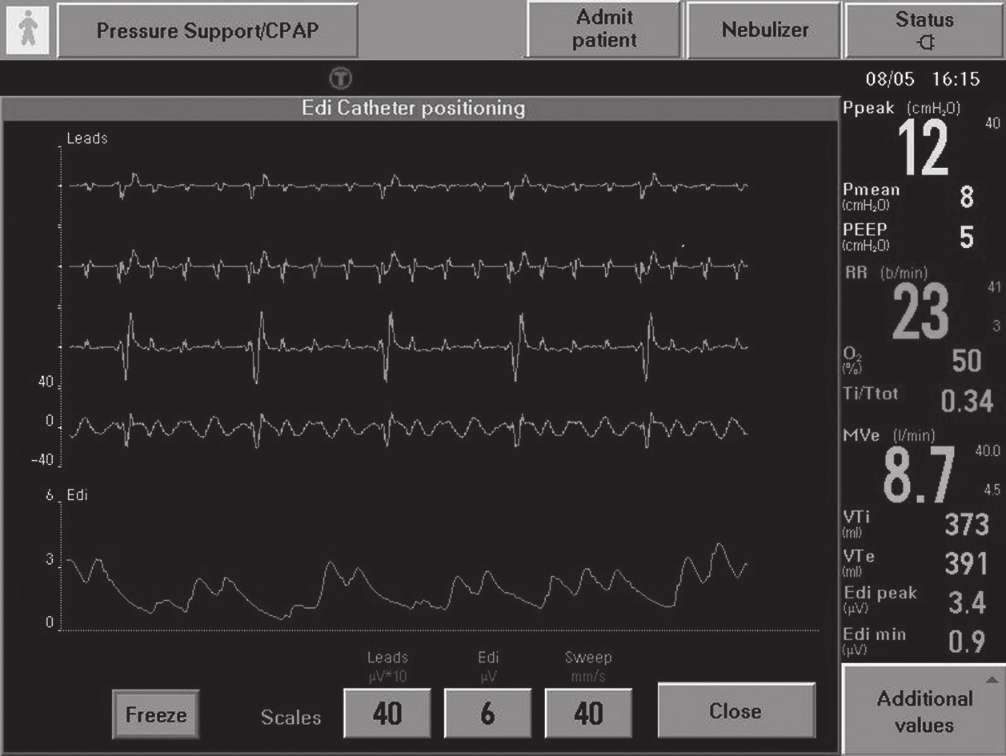
\includegraphics[width=4.5cm]{Somers/Somers-arrythmia} \&
			|[label=right:BIA]| 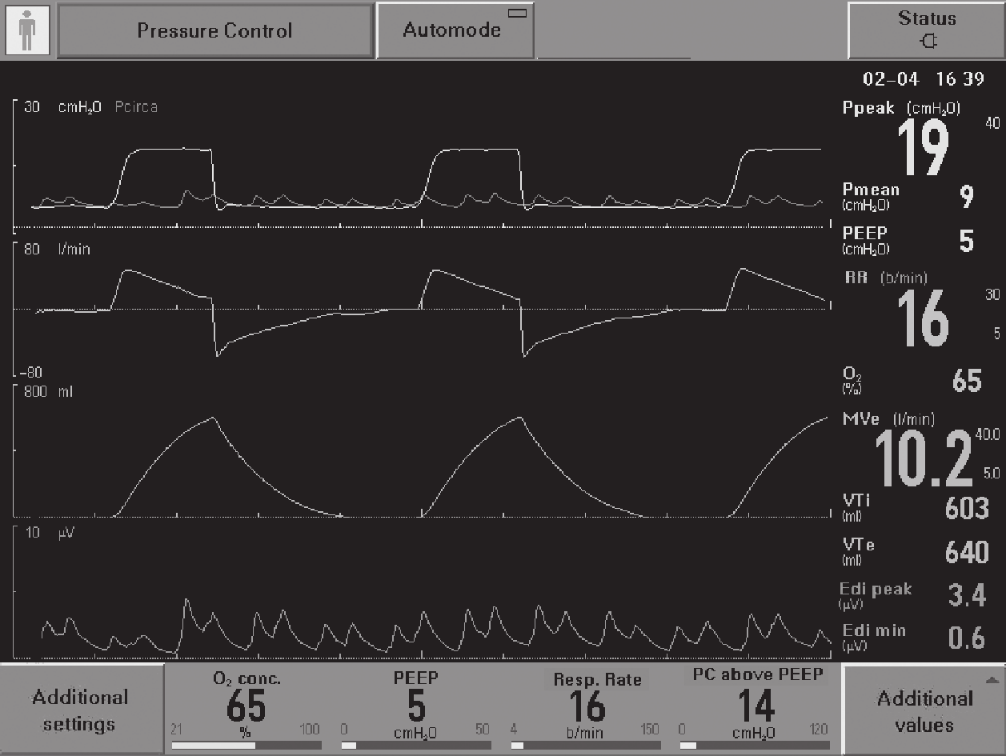
\includegraphics[width=4.5cm]{Somers/Somers-balloon} \\
			|[label=left:Chauffe-patient]|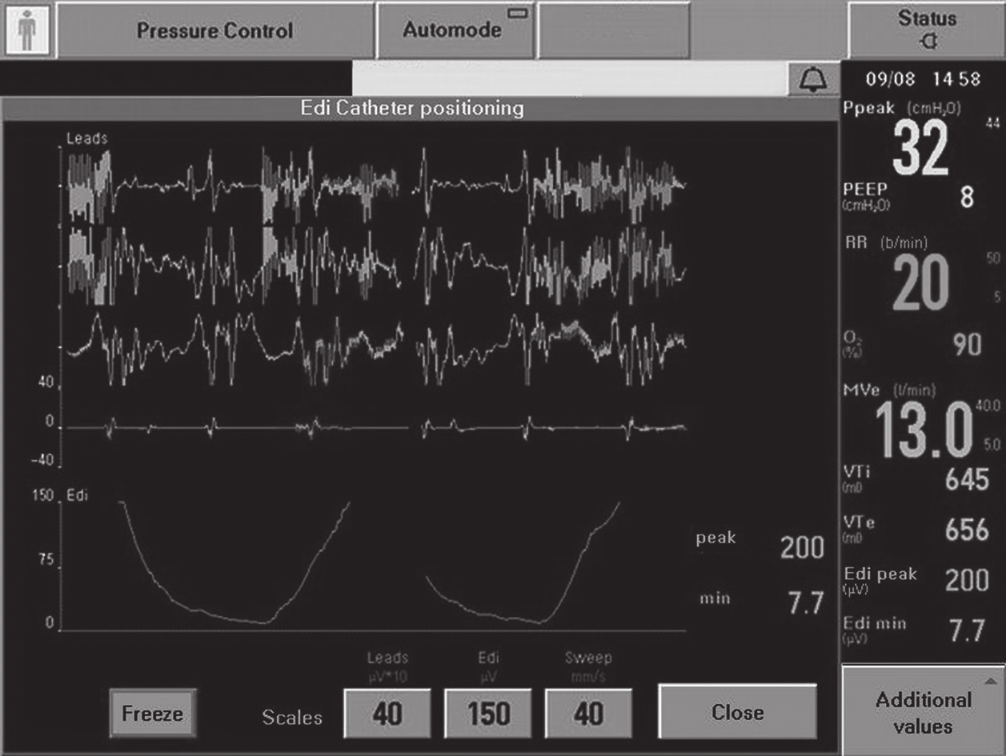
\includegraphics[width=4.5cm]{Somers/Somers-warmer} \&
			|[label=right:Stimul. card.]| 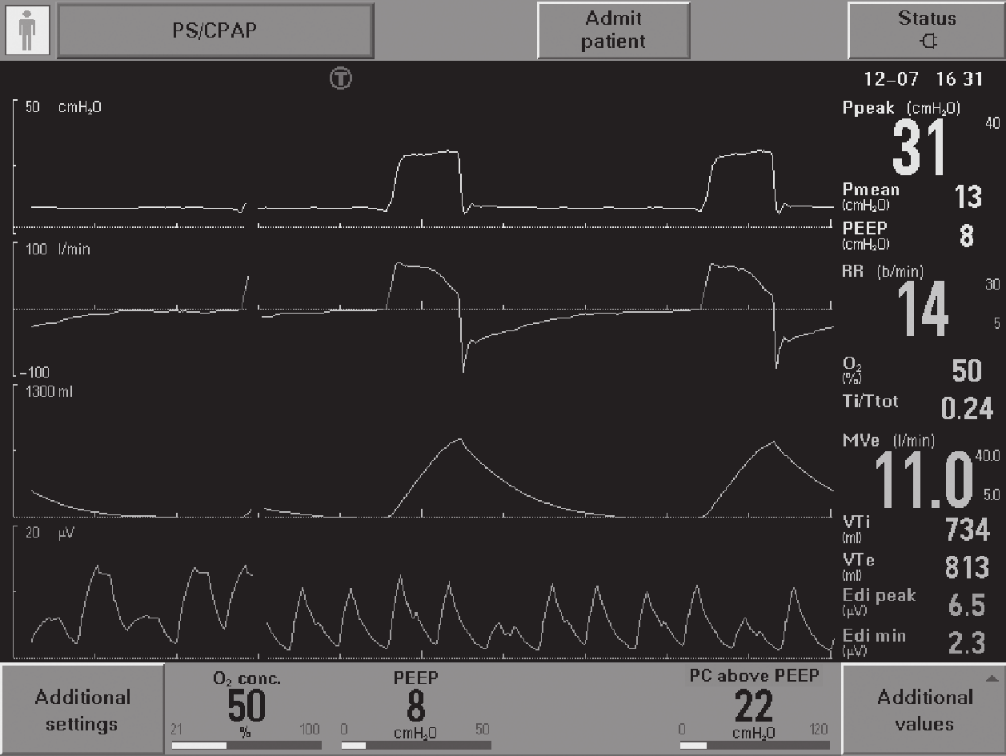
\includegraphics[width=4.5cm]{Somers/Somers-pacemaker} \\
		};

	\end{tikzpicture}\tire{somers_mechanical_2013}
\end{frame}


\section{Perte de signal}

\def\pointa{57.5}
\def\pointb{60}

\begin{frame}{La zone d'ombre du NAVA}
	\begin{tikzpicture}[]
		\begin{groupplot}[
			discrete axis,
			height=0.32\textheight,
			plot graphics/includegraphics={clip, trim=0 0 90 0},
			plot graphics/xmin=0,
			plot graphics/xmax=100,
			group style={
				group size=1 by 4,
				vertical sep=5mm,
				x descriptions at=edge bottom
			}
			]
			\nextgroupplot[paw]
			\addplot graphics[ymin=0, ymax=30]{jonkman/jonkman_a_paw-0_30};
			\coordinate (A) at(axis cs:\pointa,30);

			\nextgroupplot[poes]
			\addplot graphics[ymin=-5, ymax=12]{jonkman/jonkman_a_poes-5_12};

			\nextgroupplot[eadi]
			\addplot graphics[ymin=0, ymax=30]{jonkman/jonkman_a_eadi-0_30};

			\nextgroupplot[emgdi]
			\addplot graphics[ymin=-150, ymax=150]{jonkman/jonkman_a_emgdi};
			\coordinate (B) at(axis cs:\pointb,\pgfkeysvalueof{/pgfplots/ymin});

		\end{groupplot}
		\fill<2>[highlight] (A) rectangle (B);
	\end{tikzpicture}\adapte{jonkman_inadequate_2020}
\end{frame}

\begin{frame}{Tache aveugle du NAVA}
	\begin{tikzpicture}[]
		\begin{groupplot}[
			discrete axis,
			xmin=17,
			no markers,
			%xmin=16,
			extra x ticks={
				1.1,
				3.8,
				6.8,
				9.85,
				12.6,
				15.75
			%	19, 19.4,
			%	21.77, 22.1,
			%	24.4, 24.82,
			%	27, 27.35
			},
			group style={
				group size=1 by 3,
				vertical sep=5mm,
				x descriptions at=edge bottom
			}
			]

			\nextgroupplot[pcirc]
			\addplot table{data/1652623189887-parsed.dat};
			\coordinate (A) at (axis cs:19, \pgfkeysvalueof{/pgfplots/ymax});
			\coordinate (C) at (axis cs:21.77, \pgfkeysvalueof{/pgfplots/ymax});
			\coordinate (E) at (axis cs:24.4, \pgfkeysvalueof{/pgfplots/ymax});
			\coordinate (G) at (axis cs:27, \pgfkeysvalueof{/pgfplots/ymax});

			\nextgroupplot[debit]
			\addplot table{data/1652623189887-parsed.dat};

			\nextgroupplot[eadi]
			\addplot table{data/1652623189887-parsed.dat};
			\coordinate (B) at (axis cs:19.4, \pgfkeysvalueof{/pgfplots/ymin});
			\coordinate (D) at (axis cs:22.1, \pgfkeysvalueof{/pgfplots/ymin});
			\coordinate (F) at (axis cs:24.82, \pgfkeysvalueof{/pgfplots/ymin});
			\coordinate (H) at (axis cs:27.35, \pgfkeysvalueof{/pgfplots/ymin});

		\end{groupplot}
		\fill<2-> [highlight] (A) rectangle (B);
		\fill<3>  [highlight] (C) rectangle (D);
		\fill<3>  [highlight] (E) rectangle (F);
		\fill<3>  [highlight] (G) rectangle (H);
	\end{tikzpicture}
\end{frame}

\imgframe{captures/220520_091549.pdf}

\begin{frame}{Discussion}

	\vspace{-2.0cm}
	\begin{minipage}{0.4\textwidth}
		\centering
	\rvnl[draw=turquoisechum, fill=turquoisechum!40]{Ok. Mais on fait
quoi avec ça ?}
	\end{minipage}
	\hspace{1.5cm}
	\begin{minipage}{0.4\textwidth}
		\vspace{4cm}
		\rvnl[]{...\\[0.3\baselineskip] {\footnotesize \em(silence
			opressant)}\\[0.3\baselineskip]  Heille, on essaie-tu le
		PAV+ ?}
	\end{minipage}%
\end{frame}

\appendix
\nocite{*}
\begin{frame}{Bibliographie}
	\printbibliography
\end{frame}


\end{document}
